\section{TP4 : Transmission non-idéale, avec trajets multiples}
\sectionmark{TP4 : Transmission non-idéale, avec trajets multiples}

\subsection{Transmission non idéale avec divers bruits réels}

\subsubsection{Introduction}

Dans la continuité des étapes précédentes, l’objectif principal de cette simulation est d'étudier le comportement du système de transmission en lui-même. Cette fois-ci, le transmetteur est bruité selon un ou plusieurs schémas de perturbations aléatoires rencontrées dans la nature. Des modèles physiques de bruit seront considérés à ce stade tels que : trajets-multiples, dispersion chromatique, bruit électronique (thermique, quantique).


\begin{figure}[H]
    \centering
    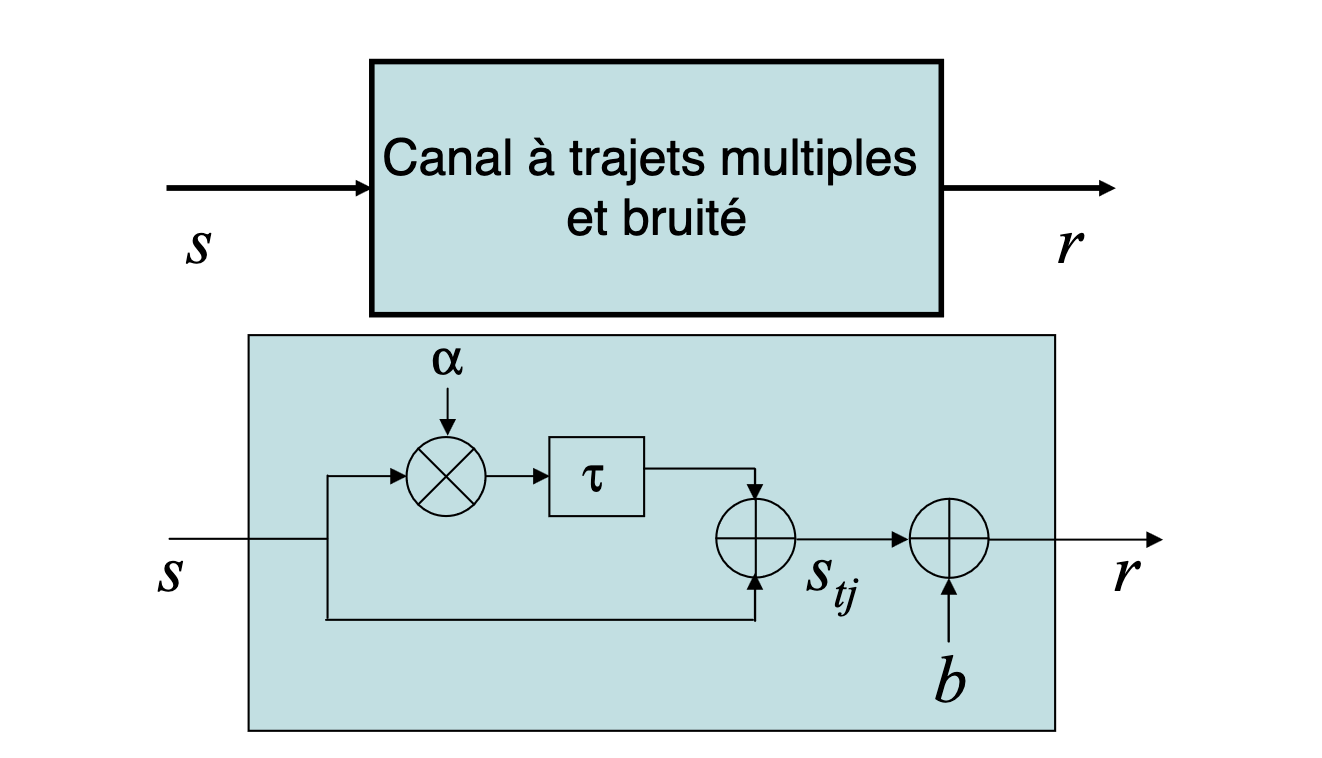
\includegraphics[width=0.7\textwidth]{img/etape4a_trajets_multiples.png}
    \caption{Trajets multiples}
    \label{fig:trajets_multiples}
\end{figure}

Nous avons précédemment implémenté une chaîne de transmission composée d'éléments analogiques et logiques, avec des CAN (Convertisseurs Analogique-Numérique) modélisant les codages NRZ, NRZT et RZ. Par la suite, nous avons réalisé des modifications de manière à ajouter bruit blanc additif gaussien (AWGN – Additive white Gaussian noise) au niveau du transmetteur, pour modéliser un comportement plus proche de la réalité. Cette nouvelle étape consistera à implémenter des signaux bruités décalés dans le temps, d'un décalage $\tau$. Cette section aura vocation à présenter les éléments pris en compte, leur implémentation dans le logiciel et une interprétation physique des résultats obtenus.

\subsubsection{Améliorations}

Avant d'aborder les explications concernant nos décisions en matière d'implémentation à l'étape 4, nous souhaitons débuter par un examen des améliorations apportées au code de l'étape 3. Pendant la phase où nous avons tracé les courbes de TEB en fonction du SNR, nous avons constaté que le simulateur était particulièrement lent lors de simulations impliquant un grand nombre de bits. Après avoir analysé notre code, nous avons observé que notre codeur NRZT (qui était le scénario le plus défavorable) avait une complexité algorithmique de l'ordre de $O(n^{3})$, tandis que les autres codeurs que nous avions mis en œuvre avaient des complexités de l'ordre de $O(n^{2})$.

Nous avons fait le choix de réécrire l'ensemble de nos codeurs afin d'obtenir une bien meilleure complexité algorithmique et pouvoir lancer des simulations sur un nombre important de bits. La réécriture des codeurs nous a permis d'atteindre une complexité algorithmique en $O(n)$ sur l'ensemble des codeurs. Cependant, cela n'a pas été une tâche aisée pour tous les codeurs, car nous avons rencontré des difficultés particulières lors de la mise en œuvre du codage NRZT. Plus précisément, les données générées ne présentaient pas les bonnes dimensions, ce qui se traduisait par une récupération incorrecte d'informations en sortie. Un problème est survenu lorsque le nombre d'échantillons par bit n'était pas divisible par 3, ce qui entraînait une perte d'échantillons.

\subsubsection{Réalisation}

\vspace{0,5cm}
Pour apercevoir les nouvelles implémentations, il faudra utiliser l'option suivante :

Le paramètre \texttt{-ti dt ar} permet l'utilisation d’une transmission analogique multi-trajets (cf . ‘trajets indirects’) :
     \begin{itemize}
        \item \texttt{dt} : précise le décalage temporel (en nombre d’échantillons) entre le trajet indirect du signal et le trajet direct
        \item \texttt{ar} : précise l’amplitude relative du signal du trajet indirect par rapport à celle du signal du trajet direct.
    \end{itemize}

\vspace{0,5cm}
Les \texttt{dt} et \texttt{ar} doivent être respectivement une valeur entière et une valeur flottante.
Plusieurs couples de valeurs (5 au maximum) peuvent être mis après le $\texttt{-ti}$ pour simuler autant de trajets indirects.
Par défaut le simulateur ne simule pas de trajets indirects, ce qui correspond à des valeurs 0 et 0,0f pour tous les trajets indirects.

La méthodologie à appliquer pour créer un signal bruité (signal blanc gaussien) étant désormais établie, nous pouvons nous focaliser sur sa mise en oeuvre. Pour cela les éléments suivants ont été implémenté :

Une classe java nommé \textbf{TransmetteurMultiTrajet}, qui permet de réaliser plusieurs trajets à l'aide de la méthode \textbf{genererSignalRetarde}, cela ajoute un décalage temporel (\texttt{dt}) pour simuler les trajets multiples avec une amplitude (\texttt{ar}) qui simule l'atténuation du signal. 

Ce n'est qu'après avoir mise en place des trajets multiples que l'on applique le bruit, cela est réalisé dans la classe \textbf{Simulateur}.

Dans notre cas, le récepteur ne connaît pas la valeur de $\tau$ et de $\alpha$, ce qui part la suite va nous poser des problèmes de performance. Si on avait voulu se placer dans un cas idéal, on serait parti du postulat que le récepteur connaissait la valeur de $\tau$ et de $\alpha$.

On pourra sûrement s'attendre à une augmentation du TEB, lors que l'on ajoutera de multiples trajts. Cela est dû à la complexité croissante du signal, à mesure que l'on ajoute des trajets. La moyenne réalisée par le récepteur devient dès lors moins précise, ce qui expliquera l'augmentation du TEB.


\begin{figure}[H]
    \centering
    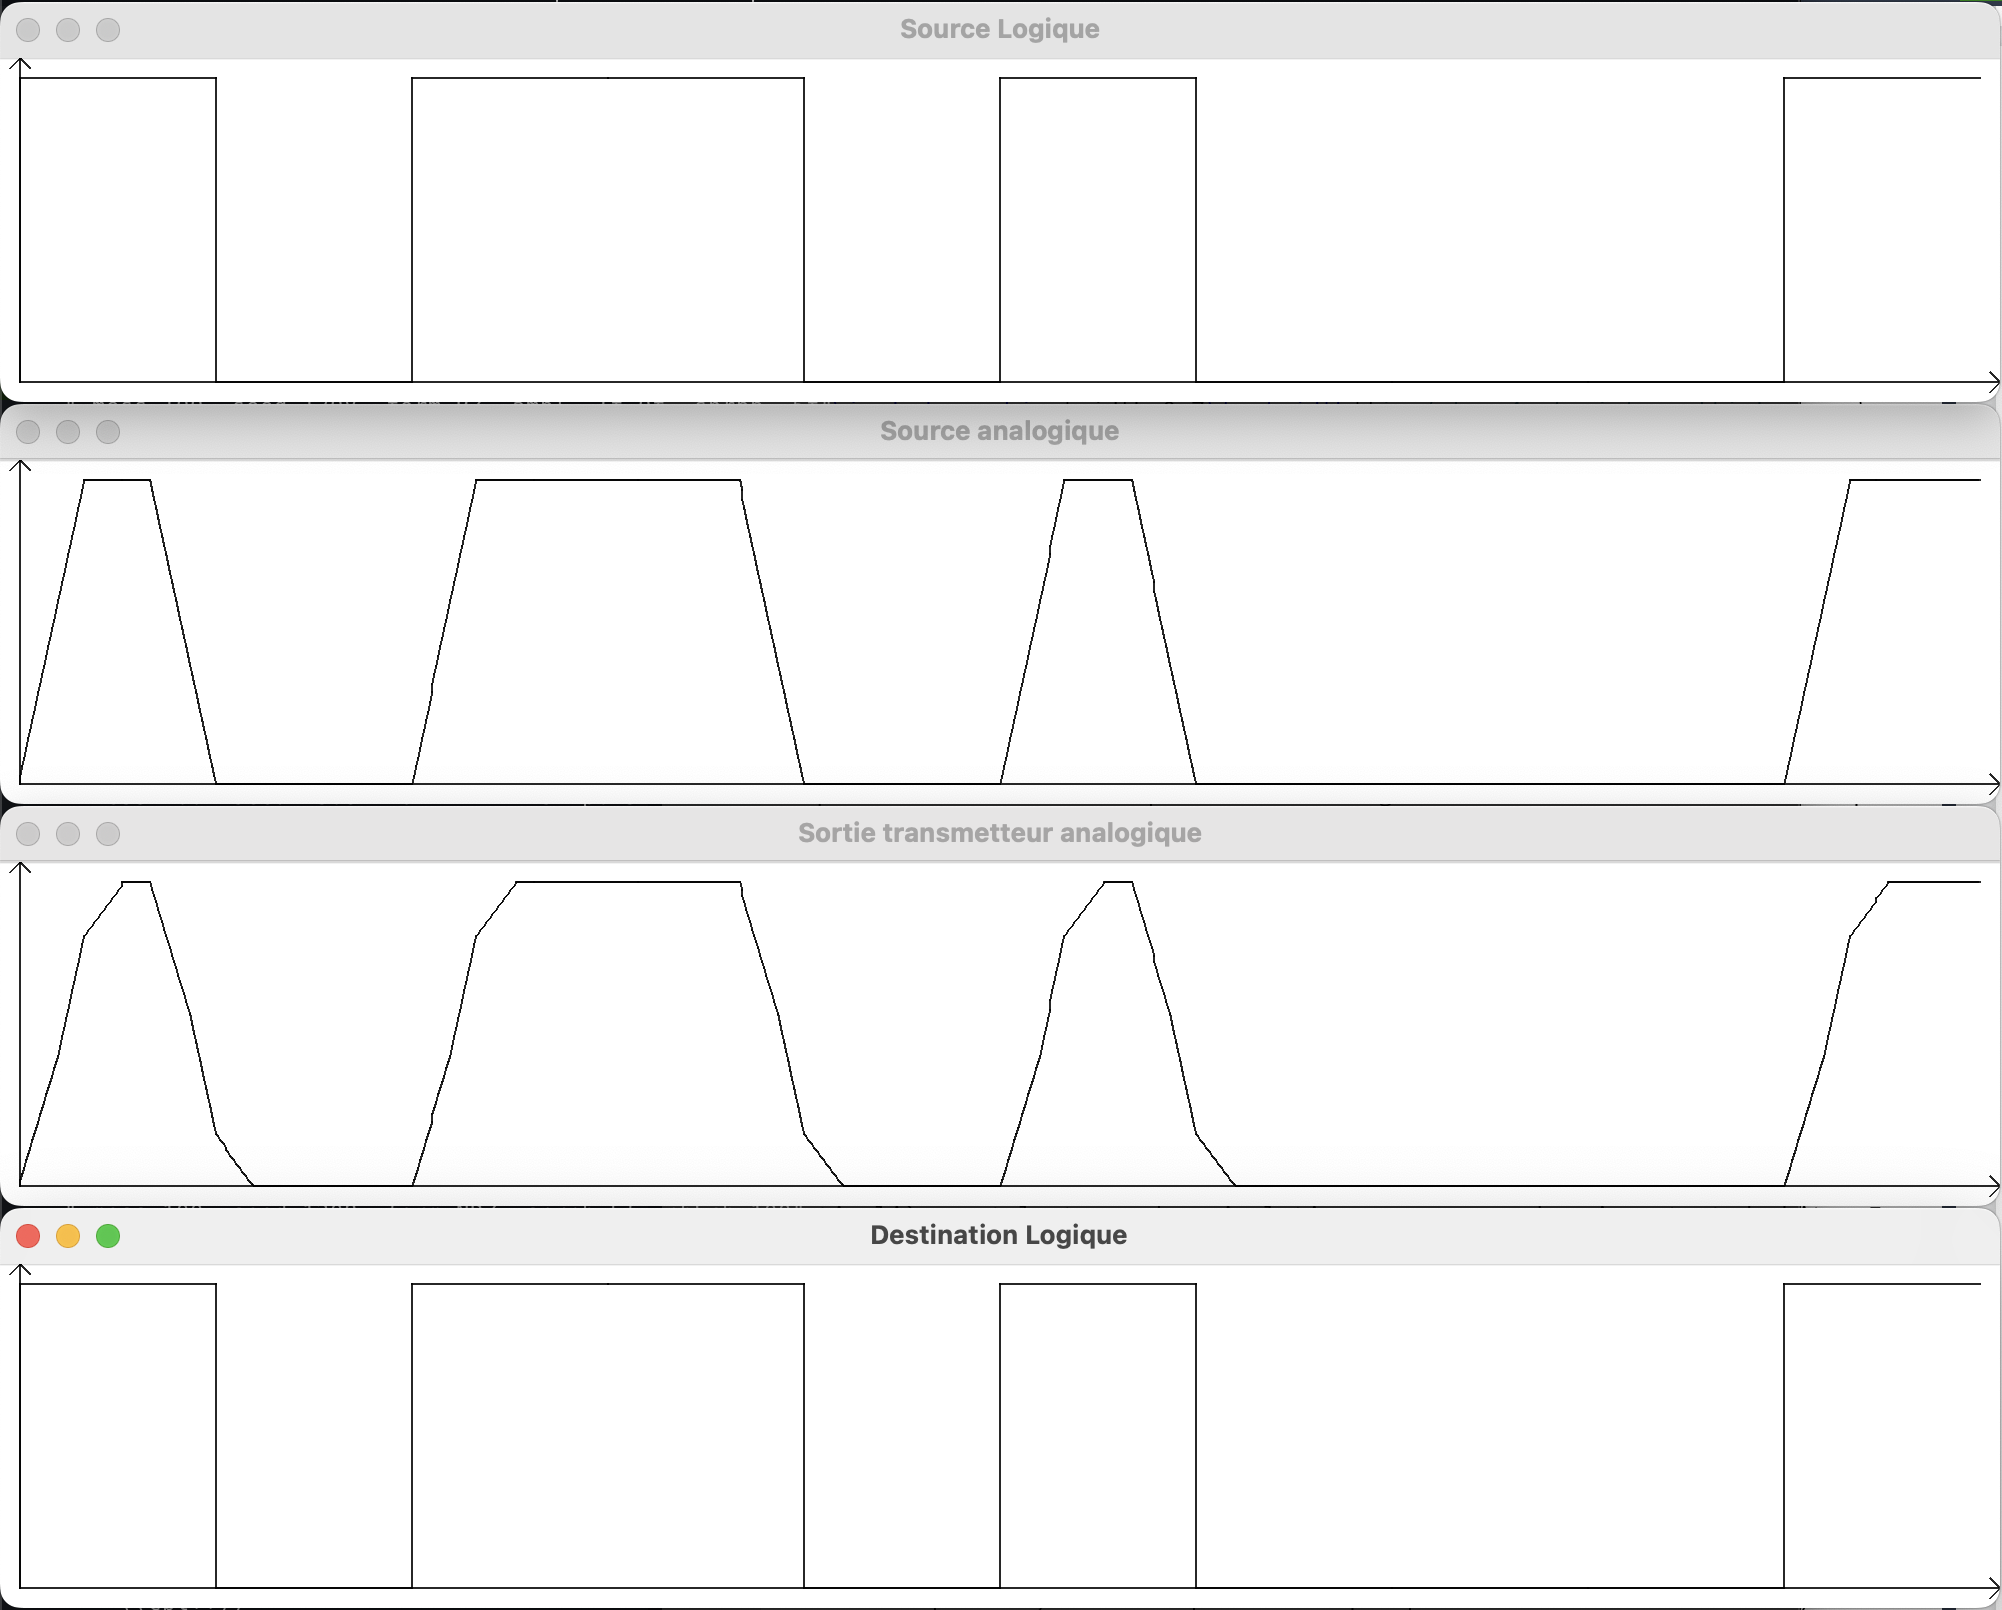
\includegraphics[width=\textwidth]{img/etape4a_ti_seul.png}
    \caption{Visualisation de la simulation NRZT (message de 10 bits avec 100 échantillons par bit) d'un trajet indirect unique sans bruit}
    \label{fig:etape4a_ti_seul}
\end{figure}

Nous avons réalisé une simulation d'un signal NRZT de 10 bits, comportant 100 échantillons. En nous basant sur ce que nous avons précédemment simulé à l'étape 2, nous pouvons constater que, du point de vue de la sonde d'émission analogique, chaque changement de valeur d'un bit logique se produit de manière progressive. On observe une pente pour la montée et la descente de chaque symbole. La différence entre la source analogique et la sortie du transmetteur analogique est très nette, et il est évident que notre signal s'est étalé dans le temps. De plus, nous observons un décalage temporel au niveau des pentes. À ce stade, notre signal de sortie du transmetteur reste clairement lisible, car nous n'avons pas encore introduit de bruit.

\begin{figure}[H]
    \centering
    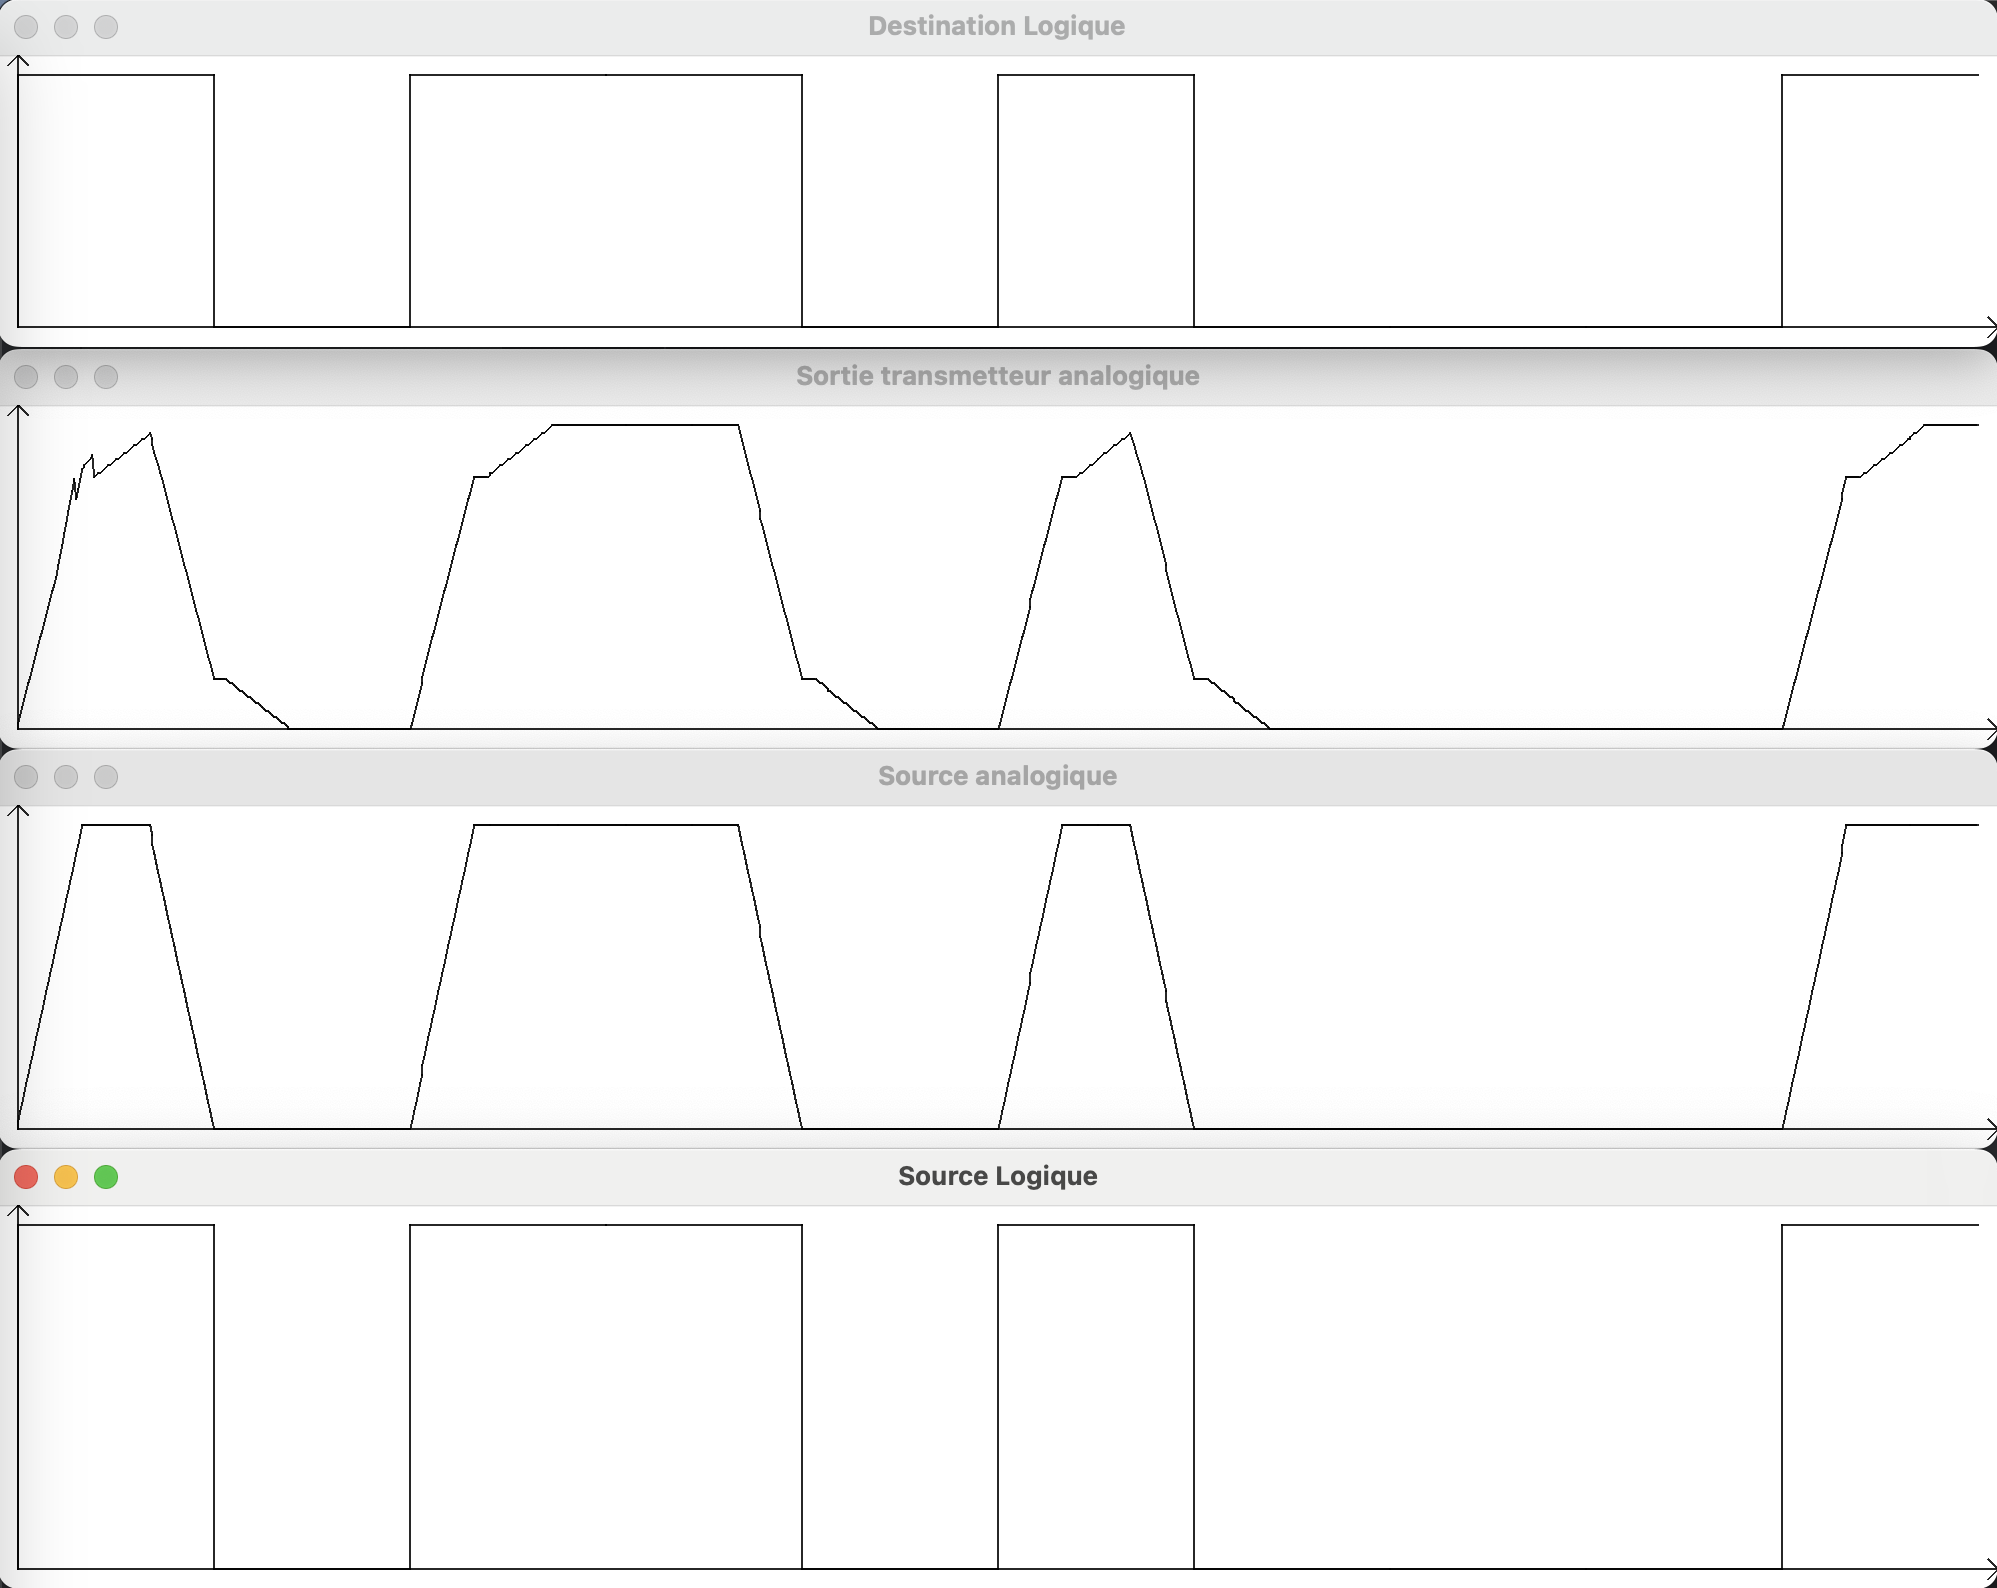
\includegraphics[width=\textwidth]{img/etape4a_ti_multiples.png}
    \caption{Visualisation de la simulation NRZT (message de 10 bits avec 100 échantillons par bit) de plusieurs trajets indirects sans bruit}
    \label{fig:etape4a_ti_multiples}
\end{figure}

Nous avons effectué une nouvelle simulation en utilisant les mêmes paramètres que ceux décrits précédemment. La seule modification apportée est l'ajout d'un nouveau signal avec un décalage temporel. Nous observons que plus nous ajoutons de trajets, plus le signal est étalé dans le temps et présente un décalage temporel significatif. Nous pouvons encore clairement distinguer les différents signaux qui ont été additionnés les uns aux autres.

\begin{figure}[H]
    \centering
    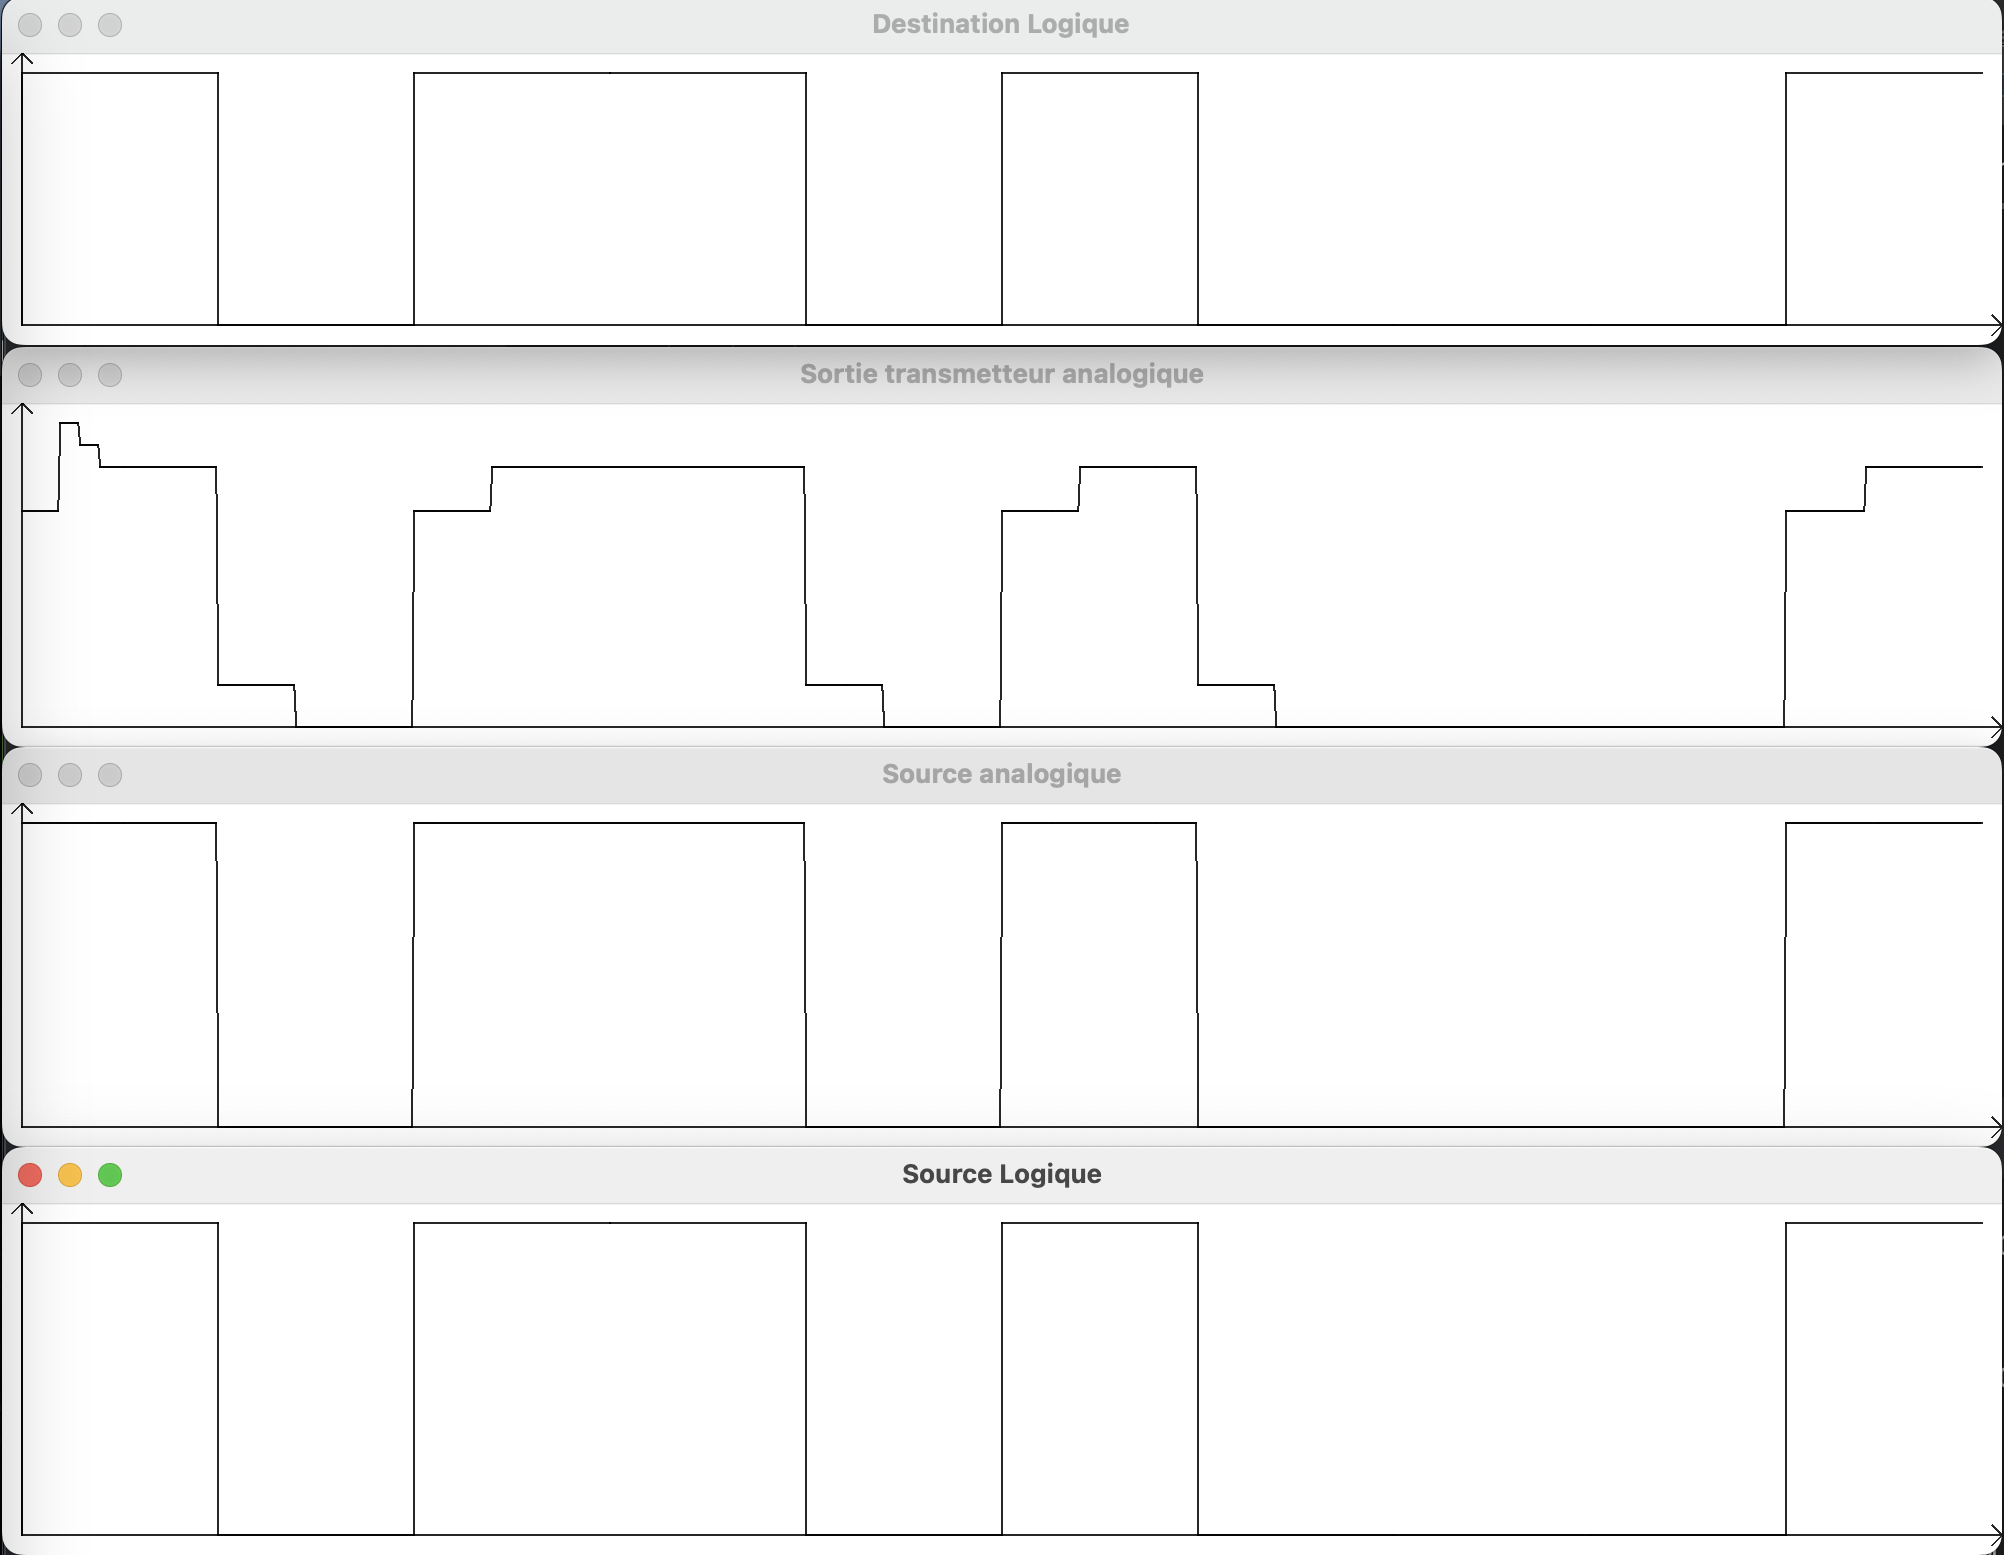
\includegraphics[width=\textwidth]{img/etape4a_ti_multiples_NRZ.png}
    \caption{Visualisation de la simulation NRZ (message de 10 bits avec 100 échantillons par bit) de plusieurs trajets indirects sans bruit}
    \label{fig:etape4a_ti_multiples_NRZ}
\end{figure}

Nous avons réalisé la simulation d'un signal bruité NRZ de 100 bits et de 100 échantillons. D'après ce que l'on a généré pour l'étape 2, on remarque bien les caractéristique du signal NRZ sur la simulation. En effet, on a bien un signal codé à l'aide de deux états, sans état intermédiaire. Pour ce qui est du transmetteur analogique en sortie, on remarque très clairement l'ajout de plusieurs signaux au signal d'origine. Particulièrement, on peut observer un étalement du symbole dans le temps, ainsi que des variations d'amplitudes pour un même symbole.

\begin{figure}[H]
    \centering
    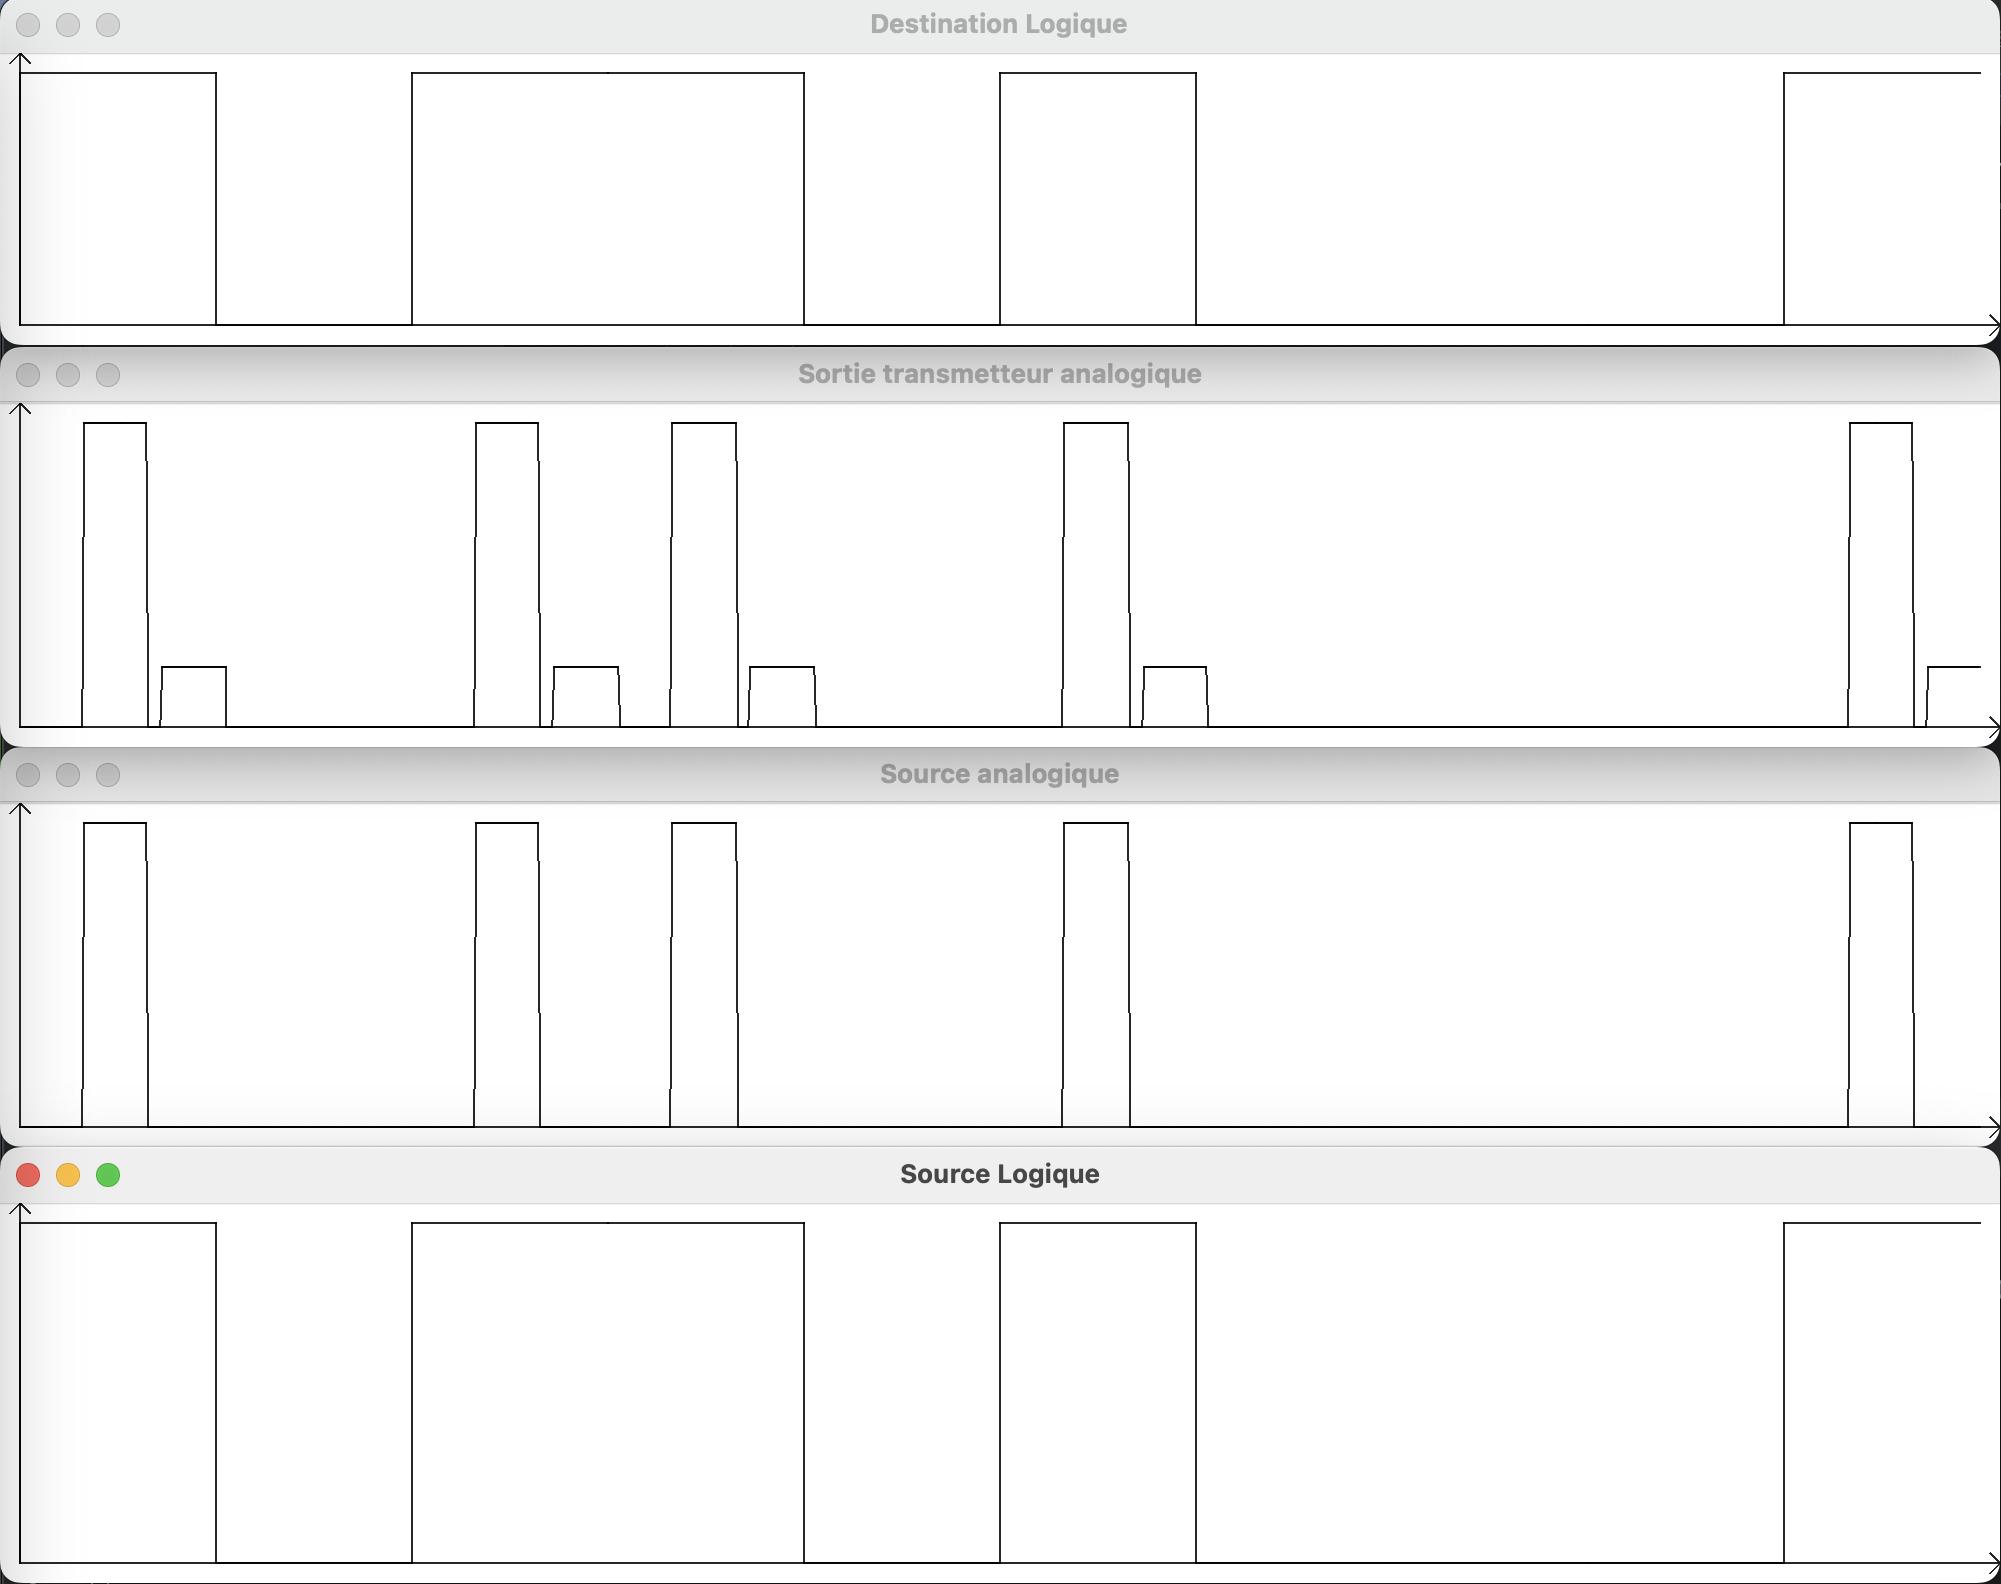
\includegraphics[width=\textwidth]{img/etape4a_ti_multiples_RZ.png}
    \caption{Visualisation de la simulation RZ (message de 10 bits avec 100 échantillons par bit) de plusieurs trajets indirects sans bruit}
    \label{fig:etape4a_ti_multiples_RZ}
\end{figure}

On a réalisé la simulation d'un signal bruité RZ de 100 bits et de 100 échantillons. D'après ce que l'on a déjà simulé à l'étape 2, on observe bien au niveau de la sonde pour l'émission analogique, chaque changement de valeur d'un bit logique est suivi d'un passage par l'état 0. Pour ce qui est du transmetteur analogique en sortie, on remarque très clairement l'ajout de plusieurs signaux au signal d'origine. Particulièrement, on peut observer un étalement du symbole dans le temps, ainsi que des variations d'amplitudes pour un même symbole.


\subsection{Transmission non idéale avec divers bruits réels et bruit gaussien}

\begin{figure}[H]
    \centering
    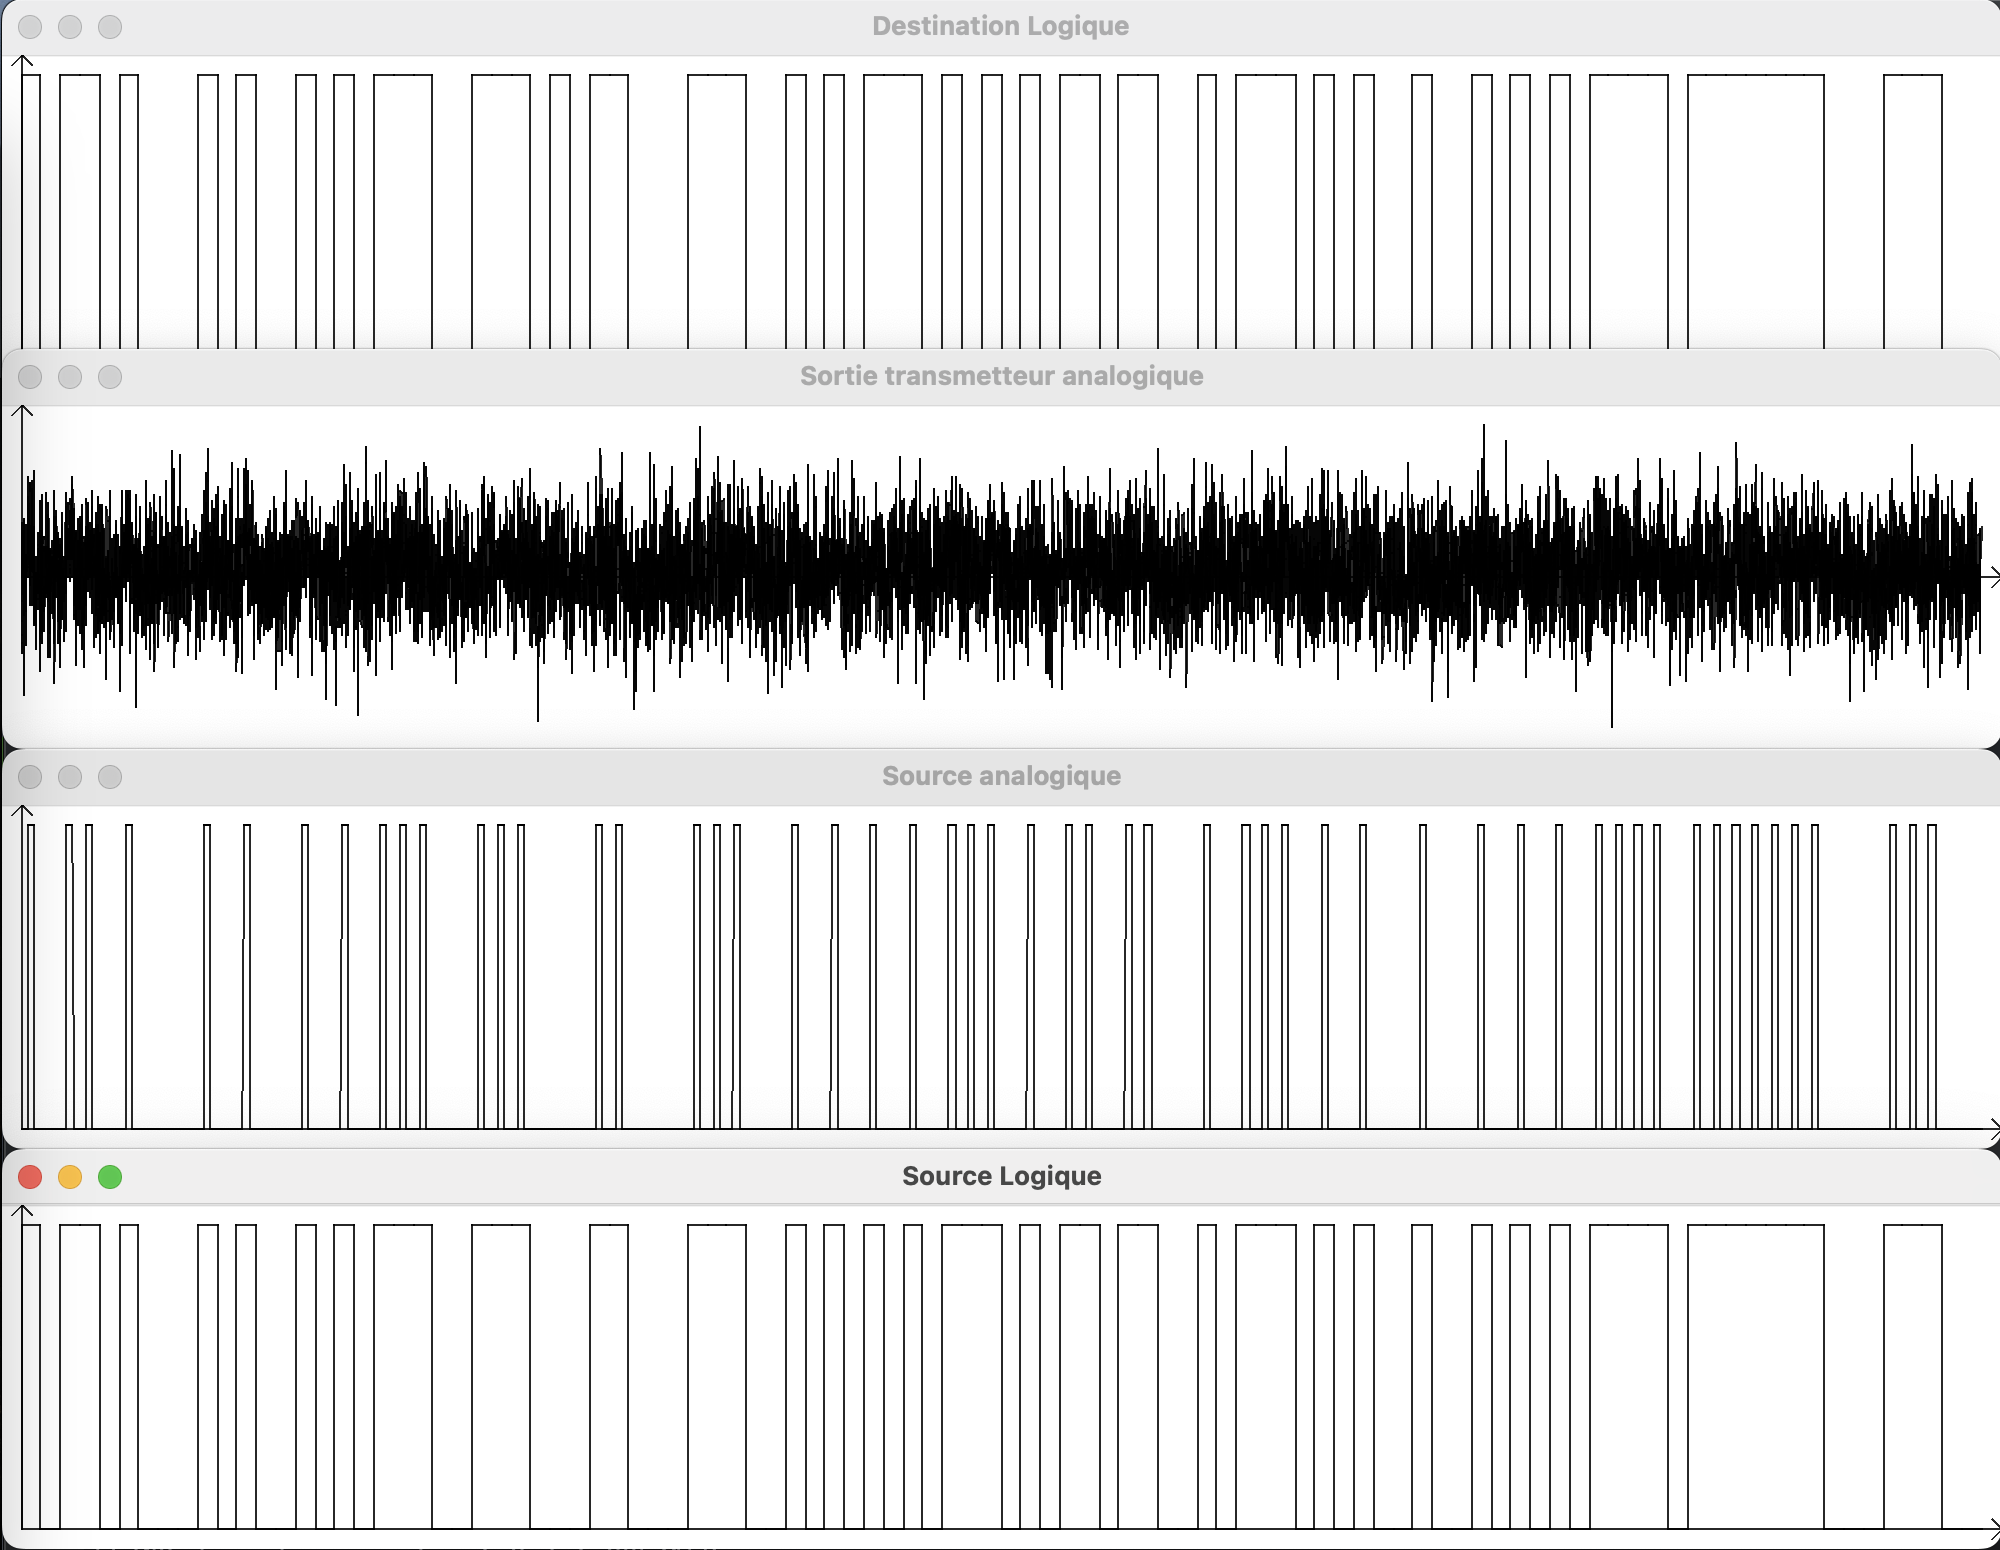
\includegraphics[width=\textwidth]{img/etape4b_ti_seul_et_bruit_6_RZ.png}
    \caption{Résultats de la simulation RZ (message de 100 bits avec 100 échantillons par bit) d'un trajet indirect unique avec un bruit de SNRpb = 6 dB}
    \label{fig:etape4b_ti_seul_et_bruit_6_RZ}
\end{figure}

Nous avons effectué la simulation d'un signal RZ bruité composé de 100 bits, de 100 échantillons et avec un rapport signal/bruit (SNR) fixé à 6 dB. Au niveau de la source analogique, nous continuons à observer notre signal présentant les caractéristiques du codage RZ que nous avons précédemment décrites. En ce qui concerne le transmetteur soumis au bruit, on observe que du bruit a été ajouté au signal d'origine. Cette perturbation entraîne des erreurs à la sortie du transmetteur, ce qui se traduit par un taux d'erreur binaire (TEB) de 0,03. Malgré l'ajout d'un trajet, nous constatons que les pertes restent très limitées.

\begin{figure}[H]
    \centering
    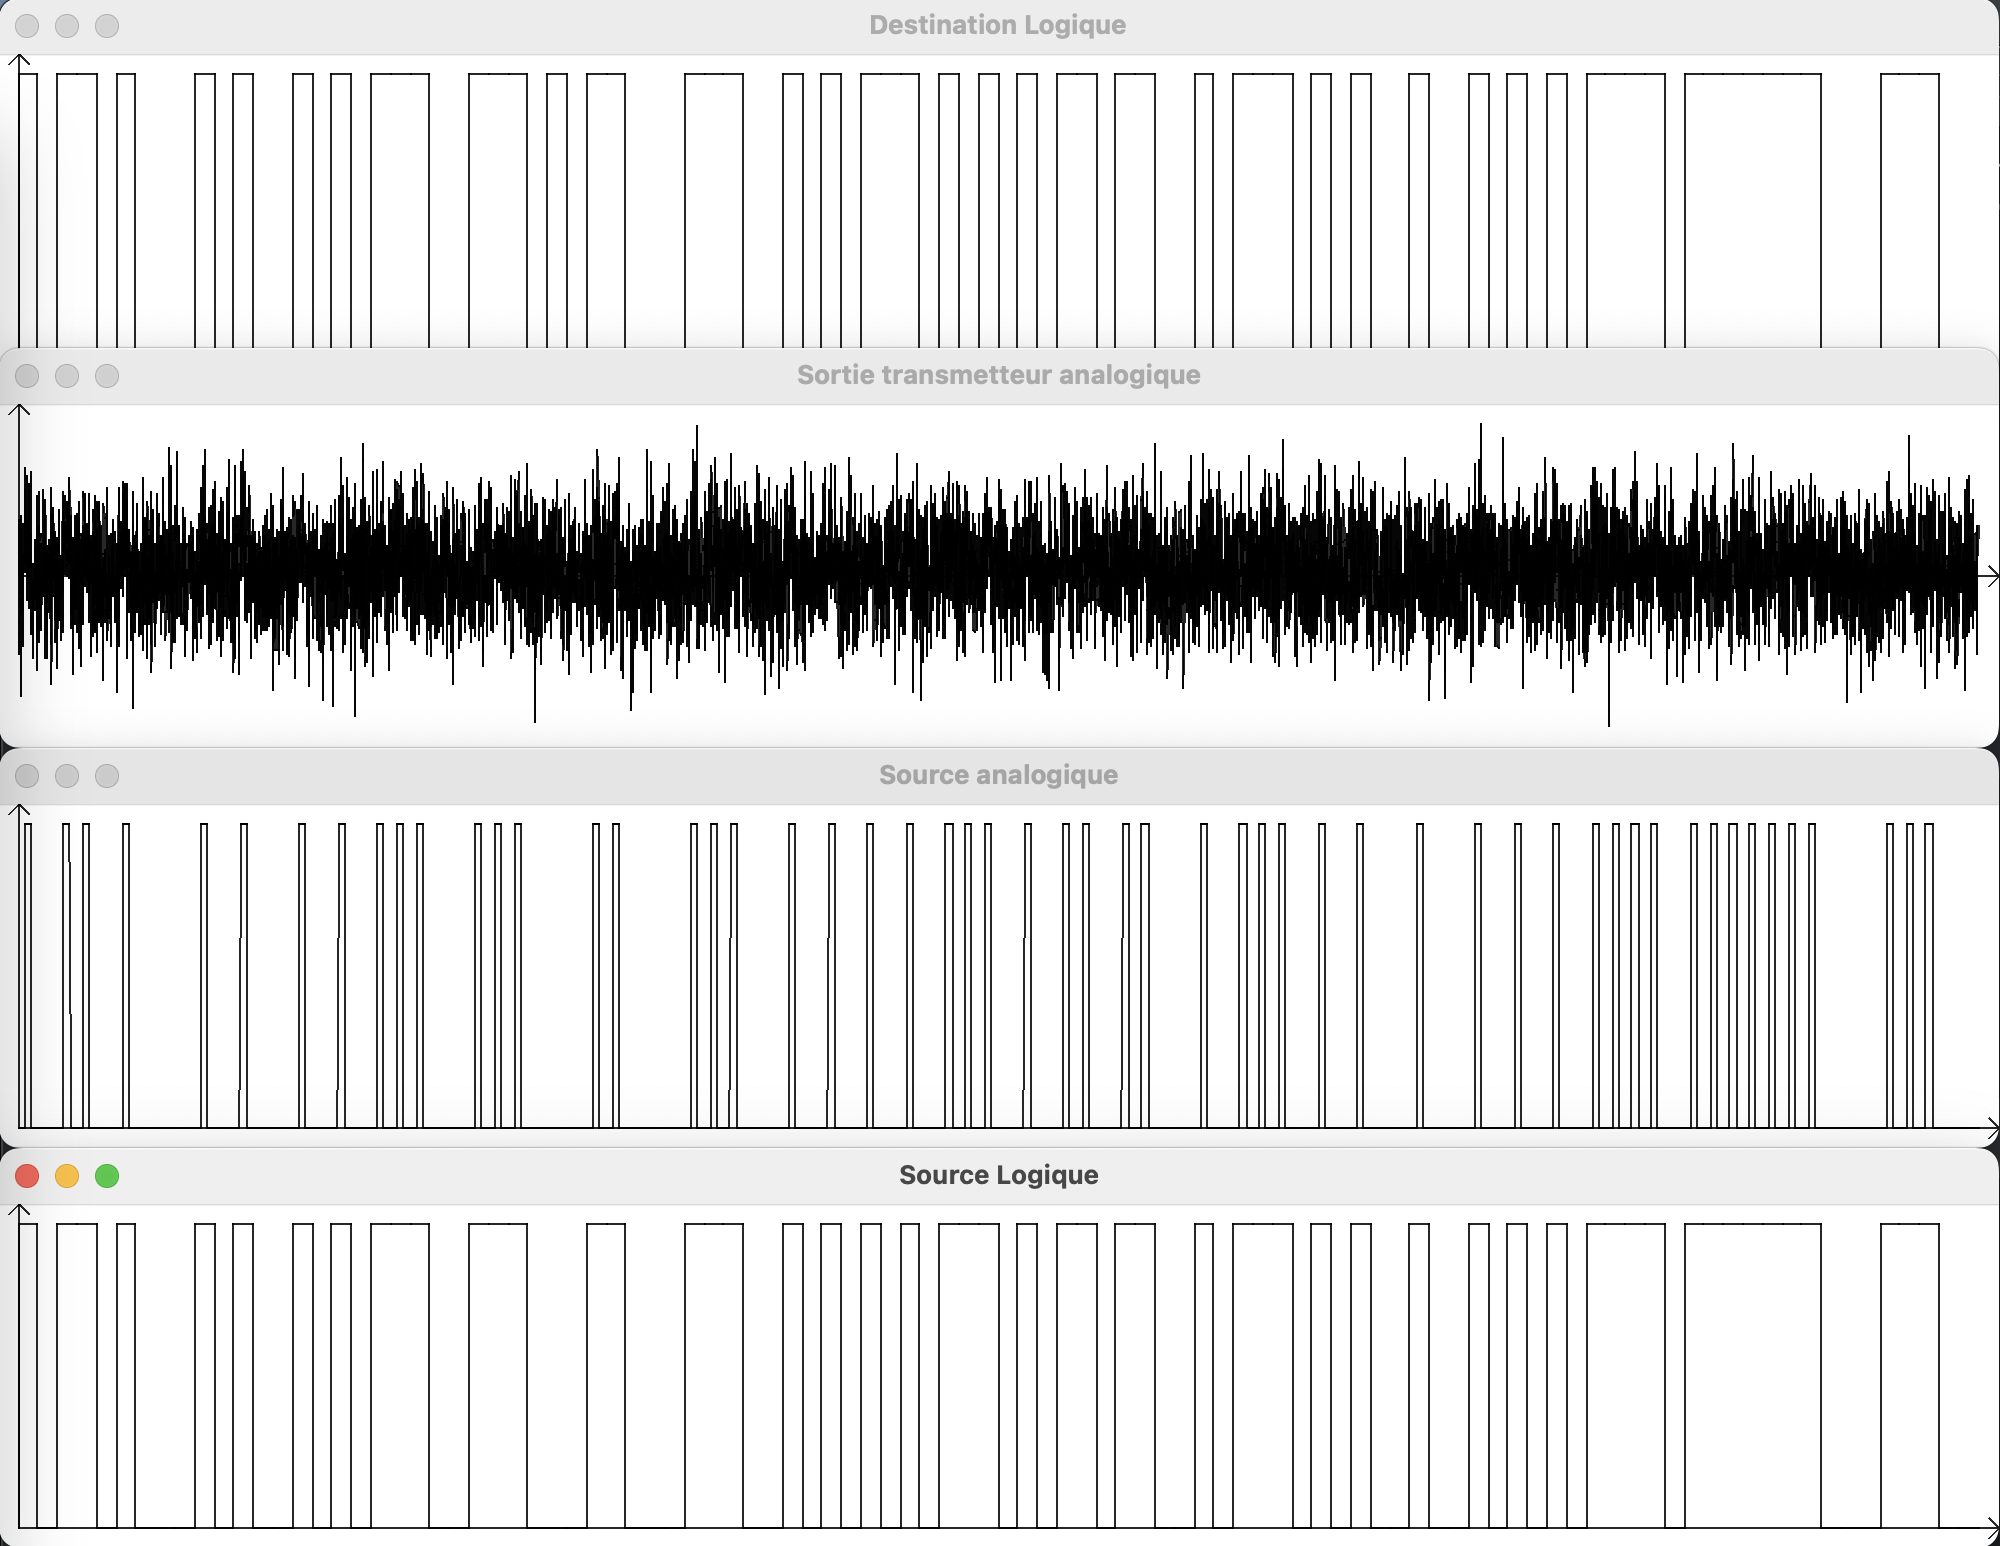
\includegraphics[width=\textwidth]{img/etape4b_ti_multiples_et_bruit_6_RZ.png}
    \caption{Résultats de la simulation RZ (message de 100 bits avec 100 échantillons par bit) de multiples trajets indirects  avec un bruit de SNRpb = 6 dB}
    \label{fig:etape4b_ti_multiples_et_bruit_6_RZ}
\end{figure}

On observe que le TEB ne varie pas malgré l'ajout de cinq trajets au signal d'origine.

\begin{figure}[H]
    \centering
    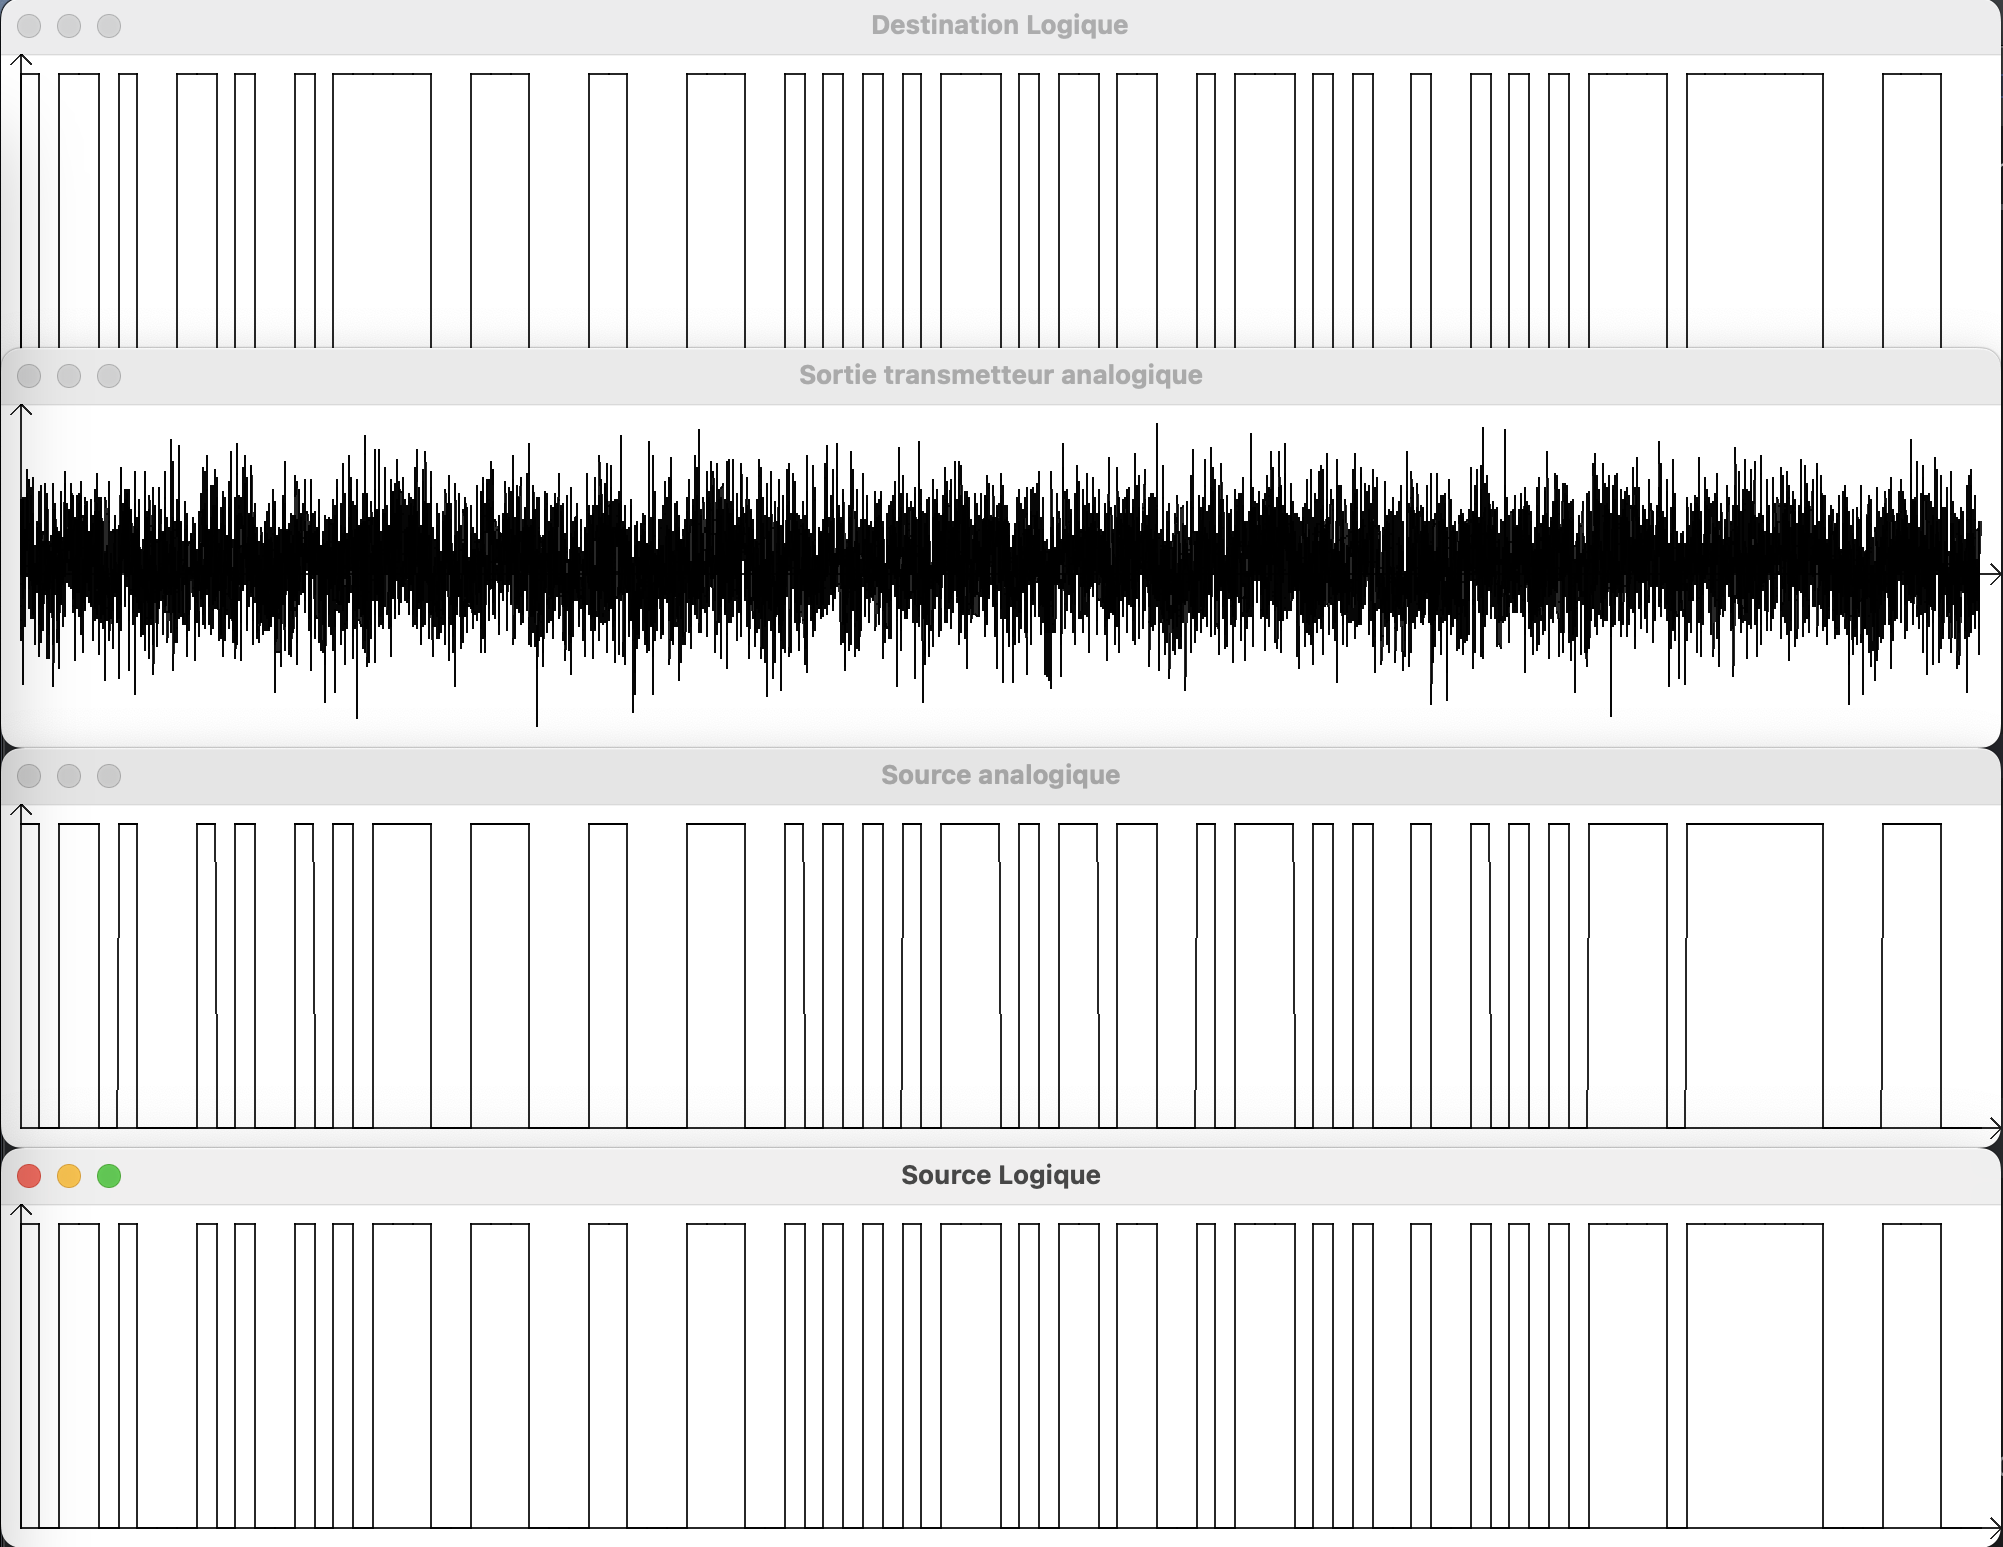
\includegraphics[width=\textwidth]{img/etape4b_ti_multiples_et_bruit_6_NRZ.png}
    \caption{Résultats de la simulation NRZ (message de 100 bits avec 100 échantillons par bit) de multiples trajets indirects avec un bruit de SNRpb = 6 dB}
    \label{fig:etape4b_ti_multiples_et_bruit_6_NRZ}
\end{figure}

Nous avons effectué la simulation d'un signal NRZ bruité composé de 100 bits, de 100 échantillons et avec un rapport signal/bruit (SNR) fixé à 6 dB. Au niveau de la source analogique, nous continuons à observer notre signal présentant les caractéristiques du codage NRZ que nous avons précédemment décrites. En ce qui concerne le transmetteur soumis au bruit, on observe que du bruit a été ajouté au signal d'origine. Cette perturbation entraîne des erreurs à la sortie du transmetteur, ce qui se traduit par un taux d'erreur binaire (TEB) de 0,02. Malgré l'ajout d'un trajet, nous constatons que les pertes restent très limitées, malgré l'ajout de cinq trajets.


\begin{figure}[H]
    \centering
    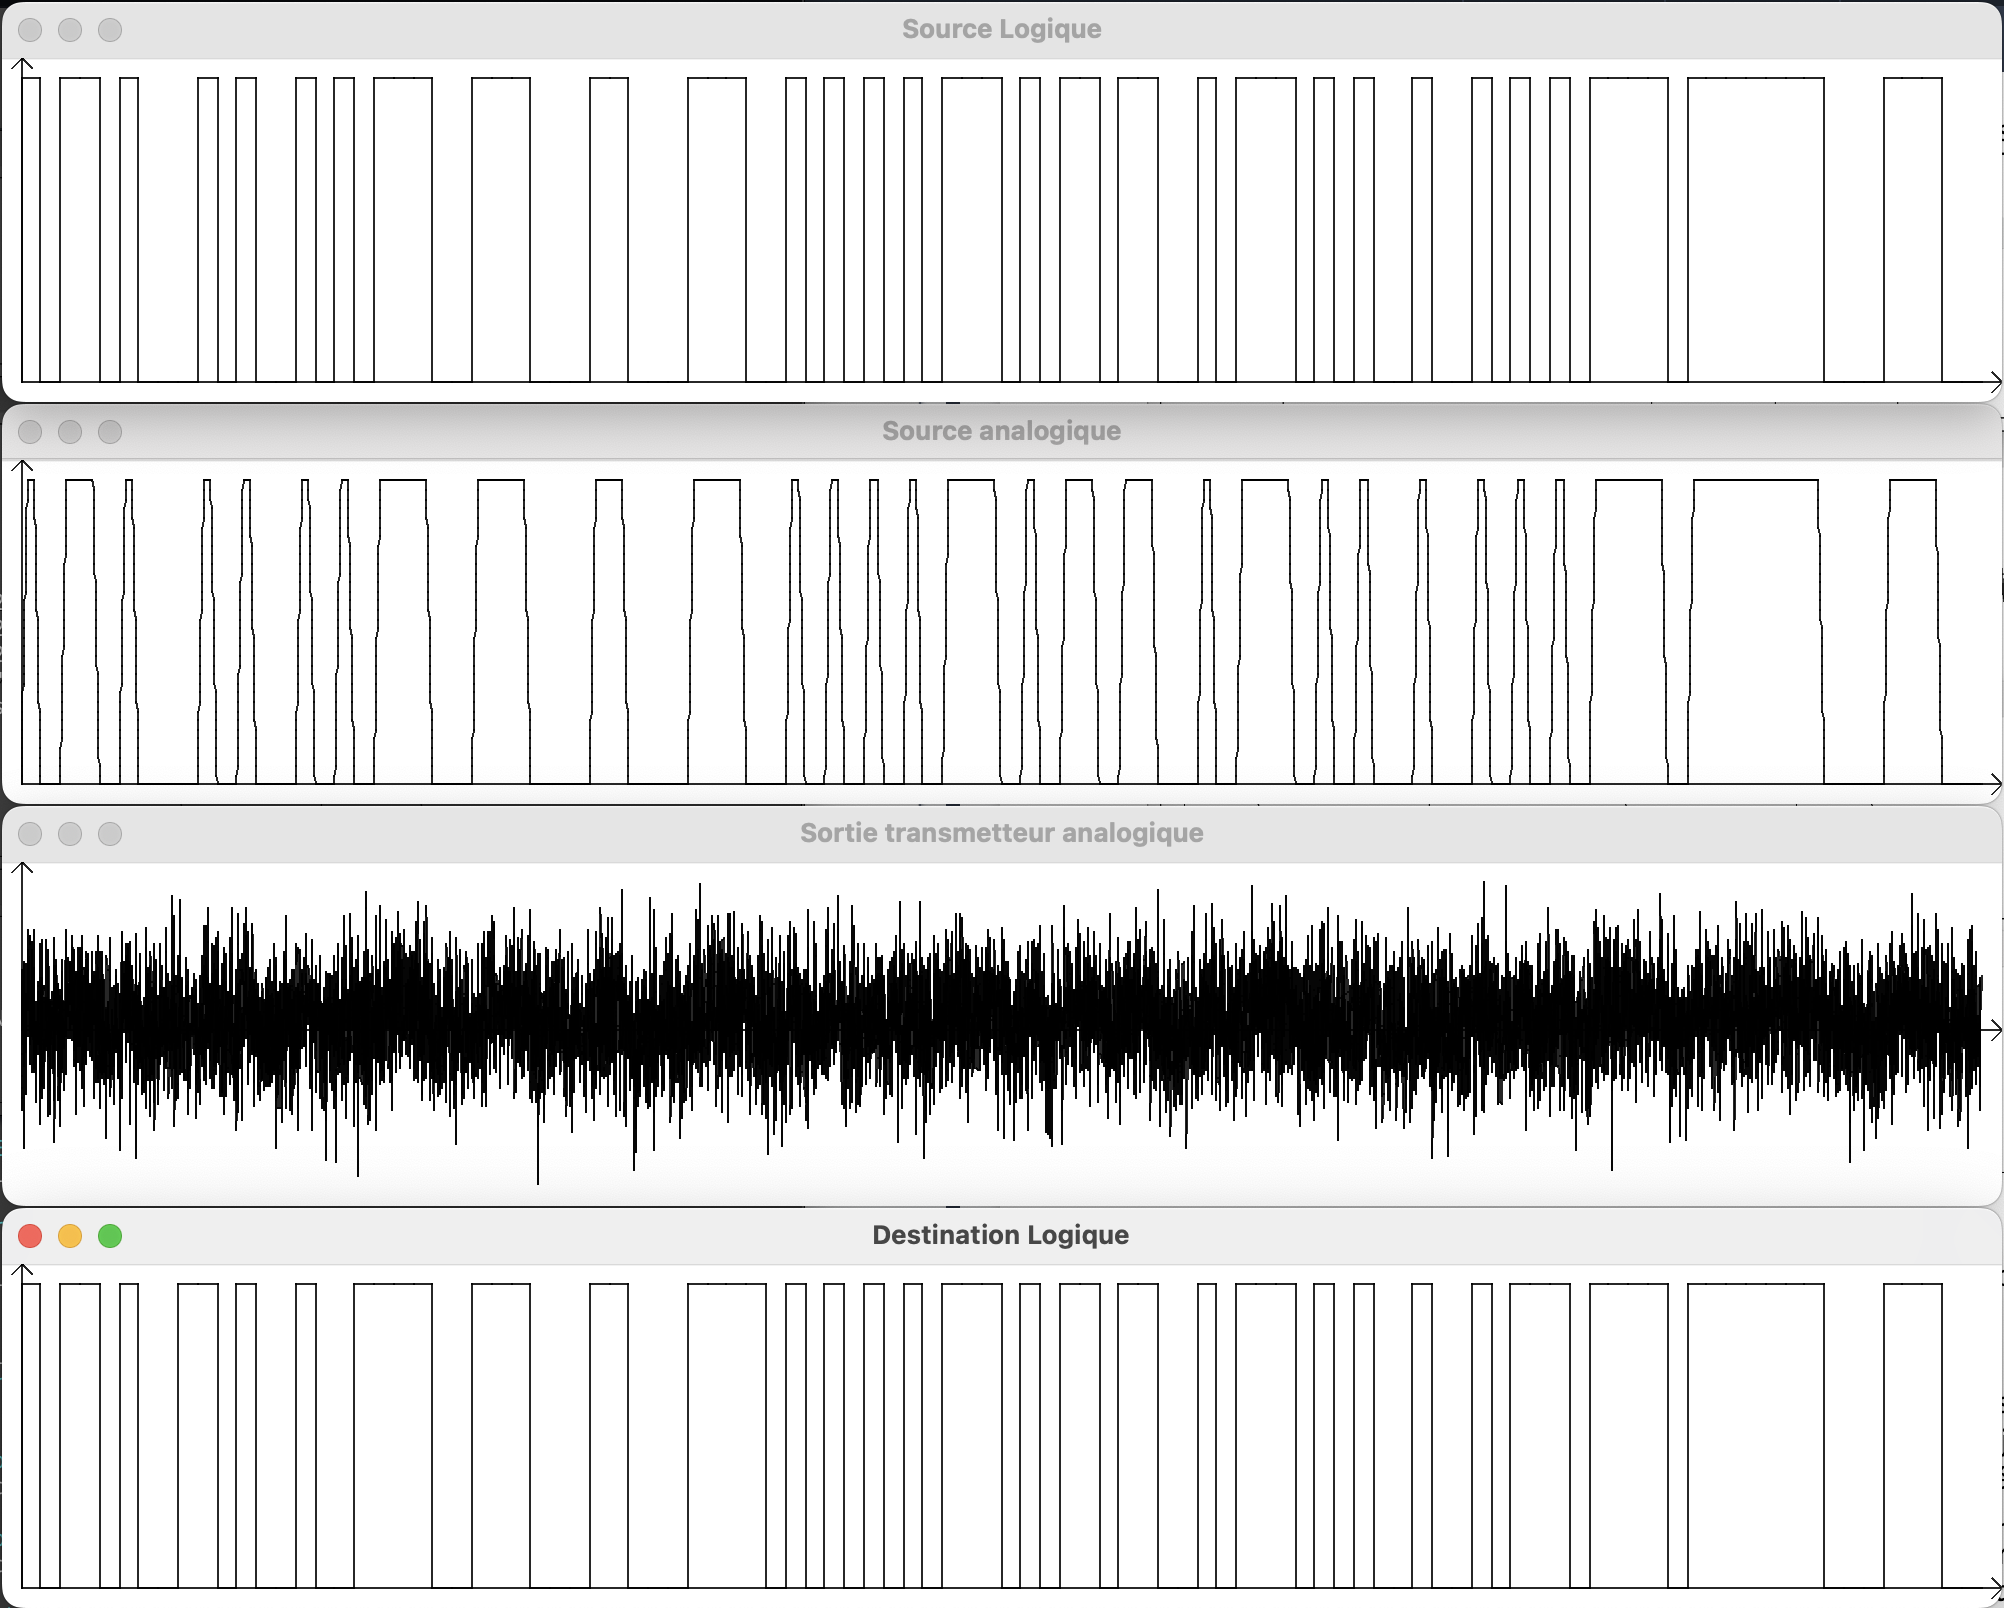
\includegraphics[width=\textwidth]{img/etape4b_ti_multiples_et_bruit_6_NRZT.png}
    \caption{Résultats de la simulation NRZT (message de 100 bits avec 100 échantillons par bit) de multiples trajets indirects avec un bruit de SNRpb = 6 dB}
    \label{fig:etape4b_ti_multiples_et_bruit_6_NRZT}
\end{figure}

Nous réalisons une simulation d'un signal bruité NRZT de 100 bits, de 100 échantillons et avec un SNR fixé à 6 dB. Au niveau de la source analogique, nous avons toujours un signal comportant les caractéristiques d'un codage NRZT, que l'on a décrit précédemment. Pour ce qui est du transmetteur bruité, on remarque très clairement l'ajout de bruit au signal d'origine. Cela va entraîner des erreurs à la sortie du transmetteur, nous constatons que le TEB a une valeur de 0,05, cela correspond à un taux d'erreur de 5$\%$. 




\subsubsection{Conclusion}

Cette étape nous a donc permis d'explorer le comportement du système de transmission en présence de divers types de bruit et de trajets multiples. Nous avons observé les effets de l'ajout de bruit sur des signaux NRZ, RZ et NRZT, en analysant leur performance en termes de taux d'erreur binaire (TEB). Nous avons observé que l’ajout de trajets multiples dans le signal – avec un décalage temporel $\tau$ – provoque un étalement du signal dans le temps. Cela peut entraîner des interférences et des distorsions dans la réception du signal, mais les pertes semblent demeurer assez limitées.

\begin{figure}[H]
    \centering
    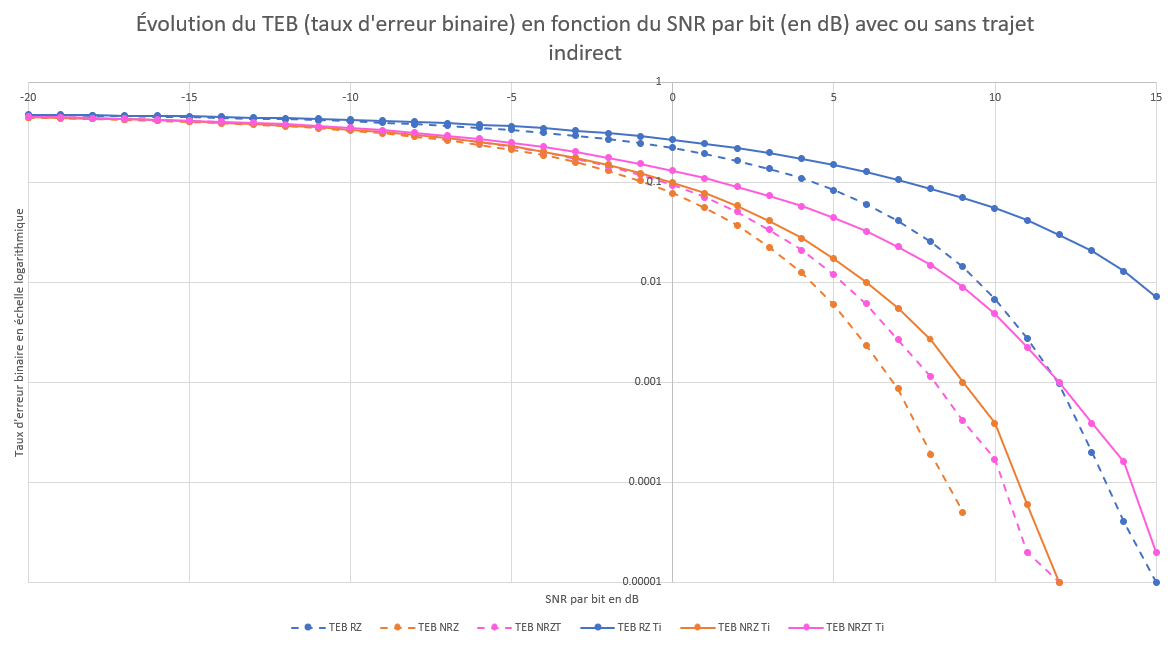
\includegraphics[width=\textwidth]{img/etape4b_teb_fct_snr_ti.png}
    \caption{Tracé du TEB en fonction du SNR par bit (semence constante, message de 100000 symboles, 30 échantillons par symbole, et trajet indirect de retard 20 échantillons et d'amplitude 0.4 fois l'amplitude du signal d'origine)}
    \label{fig:etape4b_teb_fct_snr_ti}
\end{figure}


Grâce à la figure \ref{fig:etape4b_teb_fct_snr_ti} on constate bien le résultat de cette étape : les trajets indirects affectent fortement le récepteur qui ne parvient plus à décoder aussi "bien" le signal d'origine par rapport aux simulations précédentes (sans trajets indirects).

La figure suivante indique le TEB en fonction du SNR pour différents types de simulations, de manière à synthétiser les effets des trajets multiples.

\begin{figure}[H]
    \centering
    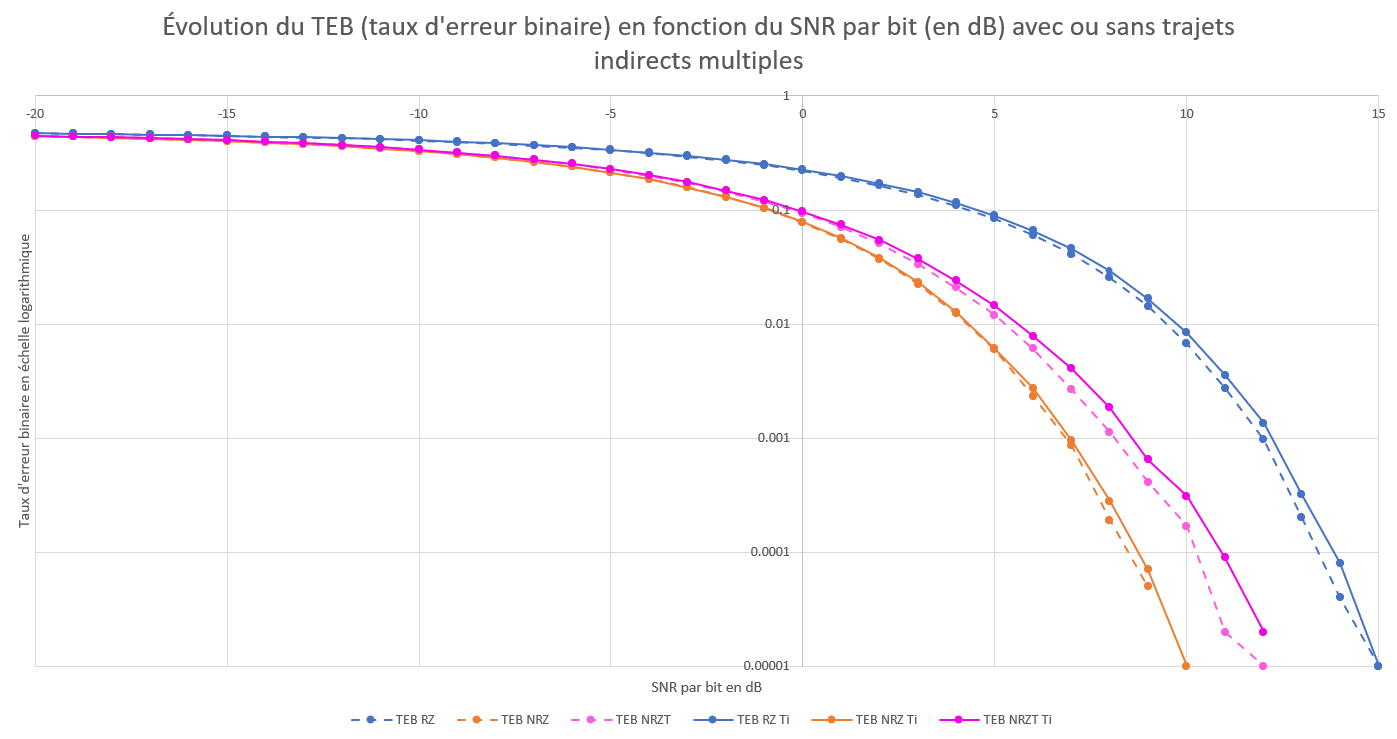
\includegraphics[width=\textwidth]{img/etape4b_teb_fct_snr_ti_multiples.png}
    \caption{Tracé du TEB en fonction du SNR par bit (semence constante, message de 100000 symboles, 30 échantillons par symbole, et trajets indirects multiples : 5/0.4 ; 10/0.25 ; 15/0.2 ; 20/0.1 ; 30/0.05)}
    \label{fig:etape4b_teb_fct_snr_ti_multiples}
\end{figure}


Cela se constate, très logiquement, beaucoup moins quand les trajets indirects ont des amplitudes relatives à l'amplitude de base plus faibles.

Dans la figure \ref{fig:etape4b_teb_fct_snr_ti_multiples} on voit bien que malgré un nombre plus important de trajets indirects (5 au lieu de 1 seul dans la figure \ref{fig:etape4b_teb_fct_snr_ti}), le décalage entre les courbes sans trajet indirect et avec trajets indirects multiples – quelle que soit la forme d'onde – sont plus proches.